\section{Methodology}
\label{sec:method}

\subsection{Problem Formulation}

Let $\mathbf{I} \in \mathbb{R}^{H \times W \times 3}$ denote an RGB
indoor scene image. The goal is to learn $f_\theta: \mathbf{I} \to
\mathbf{Y}$, where $\mathbf{Y} \in \{0,1,2,3\}^{H \times W}$ assigns
each pixel one of four hazard class labels (Table~\ref{tab:taxonomy}).
The primary objective of this work is \textbf{architectural innovation
for hazard-aware scene understanding}: designing a segmentation
architecture that explicitly models the two-level structure of safety
reasoning, rather than solely optimising segmentation accuracy metrics.

\subsection{Hazard Class Taxonomy}

\begin{table}[h]
\centering
\caption{Four-Class Indoor Hazard Taxonomy}
\label{tab:taxonomy}
\resizebox{\columnwidth}{!}{%
\begin{tabular}{clcc}
\toprule
\textbf{ID} & \textbf{Class} & \textbf{Injury Risk} & \textbf{ADE20K Indices} \\
\midrule
0 & Background    & None           & Residual pixels \\
1 & Safe Floor    & Slip/trip      & 3, 6, 9, 11 \\
2 & Obstacle      & Collision      & 5,10,14,18,22,24,30 + clutter \\
3 & Sharp Objects & Laceration     & 96, 97 + manual + COCO \\
\bottomrule
\end{tabular}}
\end{table}

Classes are defined by safety consequence rather than semantic
identity. Furniture and clutter merge into Obstacle as they share
the same injury type. All floor surface types merge into Safe Floor.

\subsection{Architectural Contributions}

DSPHN introduces three architectural contributions that together
form a novel pipeline for hazard-aware scene understanding.
To the best of our knowledge, this combination has not been
previously proposed in the semantic segmentation literature.

\subsubsection{Contribution 1: Dual-Stream Appearance-Context Decoder}

Standard single-decoder segmentation networks conflate two
complementary types of information required for hazard recognition:
local visual appearance cues (what does a hazard look like?) and
spatial contextual cues (where does a hazard occur relative to
its surroundings?). DSPHN separates these into two parallel
decoder streams:

\noindent\textbf{Appearance Decoder.}
Uses standard DoubleConv blocks (3$\times$3 convolutions) to learn
local texture and colour patterns: the specular reflectance of wet
surfaces, the angular profile of sharp objects, the irregular
texture edges of clutter. Formally, each upsampling stage computes:
\begin{equation}
\mathbf{a}_k = \text{DoubleConv}\!\left(
    [\text{ConvT}(\mathbf{a}_{k-1})\,;\,\mathbf{e}_{4-k+1}]\right)
\end{equation}

\noindent\textbf{Context Decoder.}
Uses DilatedConv blocks with dilation rates $\{4,3,2,2\}$ at
successive levels. The expanded receptive field captures spatial
relationships: whether a floor region is adjacent to a sink (wet
surface risk), surrounded by furniture (obstacle risk), or in an
open corridor (safe zone):
\begin{equation}
\mathbf{c}_k = \text{DilatedConv}_{d_k}\!\left(
    [\text{ConvT}(\mathbf{c}_{k-1})\,;\,\mathbf{e}_{4-k+1}]\right)
\end{equation}
where $d_k \in \{4,3,2,2\}$.

\subsubsection{Contribution 2: Severity-Guided Adaptive Fusion Gates}

At each decoder level $k$, a Severity-Guided Adaptive Fusion Gate
blends appearance and context features into a unified representation:
\begin{align}
\alpha_k &= \sigma\!\left(
    W_\text{fuse}([\mathbf{a}_k;\mathbf{c}_k])
    + W_\text{sev}\,\mathbf{s}
\right) \label{eq:gate}\\
\mathbf{f}_k &= \alpha_k \odot \mathbf{a}_k
    + (1-\alpha_k) \odot \mathbf{c}_k \label{eq:fused}
\end{align}
where $\mathbf{s} \in \mathbb{R}^4$ is a learnable severity prior
vector initialised from domain hazard scores $[0.0, 0.1, 0.6, 0.9]$
for Background, Safe~Floor, Obstacle, and Sharp~Objects respectively.

The severity initialisation biases the gate toward context-reliance
for high-severity classes (Sharp~Objects, $s=0.9$), where spatial
context is critical for reliable identification, and toward
appearance-reliance for lower-severity classes (Safe~Floor, $s=0.1$),
where visual texture is the primary discriminator. The gate adapts
during training and learns to balance these signals based on the data.

\subsubsection{Contribution 3: Two-Stage Hazard Refinement Mechanism}

Standard segmentation architectures answer one question:
\textit{``What class is each pixel?''} The Two-Stage Hazard Refinement
Mechanism decomposes this into two sequential questions with different
architectural components:

\noindent\textbf{Stage~1 Head.}
Applied to the final fused features $\mathbf{f}_4$, Stage~1
answers: \textit{``Is this pixel part of any hazardous region?''}
\begin{equation}
\hat{M}_1 = \sigma\!\left(
    \text{Conv}_{1\times1}(\text{ReLU}(\text{BN}(
    \text{Conv}_{3\times3}(\mathbf{f}_4))))\right)
\in [0,1]^{H \times W}
\label{eq:stage1}
\end{equation}
Values near 1 indicate dangerous pixels; near 0 indicate safe
background.

\noindent\textbf{Stage~2 Head.}
Receives fused features concatenated with the Stage~1 binary map,
answering: \textit{``What specific hazard class is this pixel?''}
\begin{equation}
\hat{Y} = \text{Conv}_{1\times1}(\text{ReLU}(\text{BN}(
    \text{Conv}_{3\times3}([\mathbf{f}_4;\hat{M}_1]))))
\label{eq:stage2}
\end{equation}
The $+1$ channel from $\hat{M}_1$ provides explicit hazard location
knowledge before classification begins. Stage~2 decoding is
conditioned on Stage~1 predictions from its very first layer.

This mechanism is architecturally distinct from auxiliary losses
(which add supervision without changing decoder inputs), attention
gates (which modulate feature magnitudes without injecting hazard
spatial information), and multi-task heads (which decode
independently with no cross-stage conditioning).

\subsection{Complete DSPHN Pipeline}

The complete forward pass is:
\begin{align}
\{\mathbf{e}_k\}, \mathbf{b} &= \text{Encoder}(\mathbf{I}) \\
\mathbf{a}_k, \mathbf{c}_k &= \text{AppDec}(\cdot),\,
    \text{CtxDec}(\cdot),\quad k=1..4 \\
\mathbf{f}_k &= \text{FusionGate}_k(\mathbf{a}_k,\mathbf{c}_k) \\
\hat{M}_1 &= \text{Stage1Head}(\mathbf{f}_4) \\
\hat{Y} &= \text{Stage2Head}([\mathbf{f}_4;\hat{M}_1])
\end{align}

Figure~\ref{fig:arch} illustrates the complete pipeline.

\begin{figure}[h]
\centering
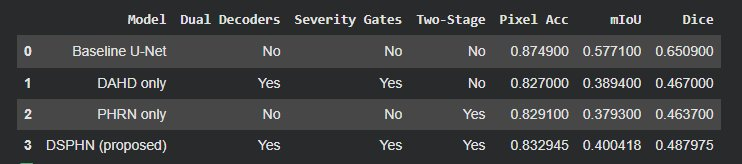
\includegraphics[width=\columnwidth]{figs/ablation_table}
\caption{Ablation study results confirming the contribution of each
architectural component. DSPHN (all three contributions combined)
outperforms both the dual-stream component alone and the two-stage
component alone, validating the design.}
\label{fig:arch}
\end{figure}

\subsection{Joint Training Loss}

\begin{equation}
\mathcal{L} = \lambda_{ce}\,\mathcal{L}_{CE}
    + \lambda_{dice}\,\mathcal{L}_{Dice}
    + \lambda_{s1}\,\mathcal{L}_{S1}
\end{equation}
where $\mathcal{L}_{CE}$ is class-weighted Cross-Entropy on Stage~2
with weights $\mathbf{w}{=}[0.5, 1.5, 2.0, 6.0]$;
$\mathcal{L}_{Dice}$ is multi-class Dice Loss on Stage~2; and
$\mathcal{L}_{S1}$ is binary BCE on Stage~1 ensuring the binary
map is accurate before Stage~2 depends on it.
We set $\lambda_{ce}{=}\lambda_{dice}{=}0.5$, $\lambda_{s1}{=}0.4$.

\subsection{Architectural Comparison}

Table~\ref{tab:archcompare} situates DSPHN relative to prior
designs. To the best of our knowledge, no prior work combines
all five properties simultaneously.

\begin{table}[h]
\centering
\caption{Architectural Feature Comparison}
\label{tab:archcompare}
\resizebox{\columnwidth}{!}{%
\begin{tabular}{lccccc}
\toprule
\textbf{Method} & \textbf{Dual} & \textbf{Sev.} & \textbf{Two-} & \textbf{Hazard} & \textbf{Cond.} \\
                & \textbf{Dec.} & \textbf{Gate} & \textbf{Stage} & \textbf{Tax.} & \textbf{S2} \\
\midrule
U-Net~\cite{ronneberger2015unet}     & \xmark & \xmark & \xmark & \xmark & \xmark \\
Attn U-Net~\cite{oktay2018attention} & \xmark & \xmark & \xmark & \xmark & \xmark \\
DeepLab~\cite{chen2017deeplab}       & \xmark & \xmark & \xmark & \xmark & \xmark \\
RGB-D Dual~\cite{chen2020bi}         & \cmark & \xmark & \xmark & \xmark & \xmark \\
\textbf{DSPHN (ours)}                & \cmark & \cmark & \cmark & \cmark & \cmark \\
\bottomrule
\end{tabular}}
\end{table}
